%%%%%%%%%%%%%%%%%%%%%%%%%%%%%%%%%%%%%%%%%%%%%%%%%%%%%%%%%%%%%%%%%%%%%%%%
\chapter{Goclassy: an Asynchronous Language Classification Pipeline for Common Crawl}\label{chap:goclassy}
%%%%%%%%%%%%%%%%%%%%%%%%%%%%%%%%%%%%%%%%%%%%%%%%%%%%%%%%%%%%%%%%%%%%%%%%

\begin{center}
    \begin{minipage}{0.66\textwidth}
        \begin{small}
            In which we present the work of \citet{ortiz-suarez-etal-2019-asynchronous}, introducing the first OSCAR corpus, now known as \emph{OSCAR 2019}, as well as asynchronous pipeline \goclassy that was used to produce OSCAR 2019 and that was specically conceived to be used in low resource infrastructures.
        \end{small}
    \end{minipage}
    \vspace{0.5cm}
\end{center}

As previously mentioned, back in the fall of 2018 when this Ph.D. started, there was no freely available contemporary French corpus of the size that was thought to be needed at that time in order to train a state-of-the art language model. The only available resources were the French Wikipedia and frWAC \citep{baroni-etal-2009-the}. At the time, the original fastText's language classification pipeline \citep{grave-etal-2018-learning} was recently published, but while \citet{grave-etal-2018-learning} published word embeddings for a wide range of languages using the produced corpus, the corpus itself was never published. We thus decided to reproduce and improve \citet{grave-etal-2018-learning} in order to get enough raw textual French data to train a language model. Given that our pipeline ended up being capable of classifying text in a wide range of languages, we decided to publish a multilingual corpus instead of a monolingual French one. In this chapter we thus lay the details of the \goclassy as well as the first version of the OSCAR corpus. 


\section{An Asynchronous Pipeline}

\begin{figure}
    \centering
    \begin{tikzpicture}[auto,scale=0.75, every node/.style={transform shape},font=\sffamily]
        \tikzstyle{nod}=[minimum width=1.65cm,minimum height=6cm,rectangle,rounded corners=10pt,
        fill=red!20, align=center, text width=1.65cm,text centered]
        \tikzstyle{ft} = [minimum width=1.5cm,minimum height=1cm,rectangle,rounded corners=10pt,
        fill=blue!20, align=center, text width=1.5cm,text centered]
        \tikzstyle{fin}=[minimum width=4cm,minimum height=4cm,rectangle,rounded corners=10pt,
        fill=green!20, align=center, text width=4cm,text centered]
        \tikzstyle{arr}=[->,>=stealth,thick]
        \tikzstyle{arr1}=[->,>=stealth,thick, dashed]

        \node[nod] (CC) at (0,0) {Common Crawl};

        \node[minimum width=2cm, text width=2cm,text centered] (TEX1) at (2.5,3.45) {\small Compressed Files};
        \node (GZ1) at (2.5,2.3) {\Huge \faFileArchive[regular]};
        \node (GZ2) at (2.5,1) {\Huge \faFileArchive[regular]};
        \node (GZ3) at (2.5, -0.3) {\Huge \faFileArchive[regular]};
        \node (DGZ) at (2.5, -1.2) {\Huge $\vdots$};
        \node (GZ4) at (2.5,-2.3) {\Huge \faFileArchive[regular]};


        \node[minimum width=1cm, text width=1cm,text centered] (TEX1) at (4.5,3.45) {\small WET Files};
        \node (T1) at (4.5,2.3) {\Huge \faFile*};
        \node (T2) at (4.5,1) {\Huge \faFile*};
        \node (T3) at (4.5, -0.3) {\Huge \faFile*};
        \node (DT) at (4.5, -1.2) {\Huge $\vdots$};
        \node (T4) at (4.5,-2.3) {\Huge \faFile*};

        \node[ft] (F1) at (7,2.3) {fastText};
        \node[ft] (F2) at (7,1) {fastText};
        \node[ft] (F3) at (7,-0.3) {fastText};
        \node (DF) at (7, -1.2) {\Huge $\vdots$};
        \node[ft] (F4) at (7,-2.3) {fastText};

        \node[minimum width=2.3cm, text width=2.3cm,text centered] (TEX1) at (10.25,3.45) {\small Filtered Files Language Tags};
        \node (TA1) at (10.25,2.3) {\Huge \faFile*[regular] $\,$ \faTags};
        \node (TA2) at (10.25,1) {\Huge \faFile*[regular] $\,$ \faTags};
        \node (TA3) at (10.25, -0.3) {\Huge \faFile*[regular] $\,$ \faTags};
        \node (DTA) at (10.25, -1.2) {\Huge $\vdots$};
        \node (TA4) at (10.25,-2.3) {\Huge \faFile*[regular] $\,$ \faTags};


        \node[minimum width=2.3cm, text width=2.3cm,text centered] (TEX1) at (15,3.45) {\small Files Classified by Language};
        \node[fin] (FF) at (15,0) {};
        \node (TF) at (15,1.3) {\Huge \faLanguage $\,\cdots$\faLanguage};
        \node (TF3) at (15, 0) {\Huge \faLanguage $\,\cdots$\faLanguage};
        \node (TF3) at (15, -1.3) {\Huge \faLanguage $\,\cdots$\faLanguage};


        \draw[arr] (1,2.3)--(GZ1);
        \draw[arr] (1,1)--(GZ2);
        \draw[arr] (1,-0.3)--(GZ3);
        \draw[arr] (1,-2.3)--(GZ4);


        \draw[arr] (GZ1)--(T1);
        \draw[arr] (GZ2)--(T2);
        \draw[arr] (GZ3)--(T3);
        \draw[arr] (GZ4)--(T4);


        \draw[arr1] (5,2.5)--(6.1,2.5);
        \draw[arr1] (5,2.3)--(6.1,2.3);
        \draw[arr1] (5,2.1)--(6.1,2.1);

        \draw[arr1] (5,1.2)--(6.1,1.2);
        \draw[arr1] (5,1)--(6.1,1);
        \draw[arr1] (5,0.8)--(6.1,0.8);

        \draw[arr1] (5,-0.1)--(6.1,-0.1);
        \draw[arr1] (5,-0.3)--(6.1,-0.3);
        \draw[arr1] (5,-0.5)--(6.1,-0.5);

        \draw[arr1] (5,-2.1)--(6.1,-2.1);
        \draw[arr1] (5,-2.3)--(6.1,-2.3);
        \draw[arr1] (5,-2.5)--(6.1,-2.5);


        \draw[arr] (8,2.5)--(9.1,2.5);
        \draw[arr] (8,2.3)--(9.1,2.3);
        \draw[arr] (8,2.1)--(9.1,2.1);

        \draw[arr] (8,1.2)--(9.1,1.2);
        \draw[arr] (8,1)--(9.1,1);
        \draw[arr] (8,0.8)--(9.1,0.8);

        \draw[arr] (8,-0.1)--(9.1,-0.1);
        \draw[arr] (8,-0.3)--(9.1,-0.3);
        \draw[arr] (8,-0.5)--(9.1,-0.5);

        \draw[arr] (8,-2.1)--(9.1,-2.1);
        \draw[arr] (8,-2.3)--(9.1,-2.3);
        \draw[arr] (8,-2.5)--(9.1,-2.5);


        \draw[arr] (TA1.0)--(FF);
        \draw[arr] (TA2.0)--(FF);
        \draw[arr] (TA3.0)--(FF);
        \draw[arr] (TA4.0)--(FF);
    \end{tikzpicture}
    \caption{A scheme of the \goclassy pipeline. The red square represents the Compressed WET files stored on Amazon Web Services. The {\faFileArchive[regular]} icons represent the gzip files stored locally, the {\faFile*} represents one of the 50K WET files. The {\faFile*[regular]} represents the filtered file and the {\faTags} represents a file of language tags, one tag per line in \faFile*[regular]. The {\faLanguage} represents one of the 166 classified files. Each arrow represents an asynchronous non-blocking worker and dotted arrows represent a line filtering process.}
    \label{fig:D1}
\end{figure}

We propose a new pipeline derived from the fastText one which we call \goclassy, we reuse the fastText linear classifier \citep{joulin-etal-2016-fasttext, joulin-etal-2017-bag} and the pre-trained fastText model for language recognition \citep{grave-etal-2018-learning}, but we completely rewrite and parallelize their pipeline in an asynchronous manner.

The order of operations is more or less the same as in the fastText pre-processing pipeline but instead of clustering multiple operations into a single blocking process, we launch a worker for each operation, and we bound the number of possible parallel operations at a given time by the number of available threads instead of the number of CPUs. We implement \goclassy using the Go programming language\footnote{\url{https://golang.org/}} so we let the Go runtime\footnote{\url{https://golang.org/src/runtime/mprof.go}} handle the scheduling of the processes. Thus, in our pipeline we don't have to wait for a whole WET file to download, decompress and classify in order to start downloading and processing the next one, a new file will start downloading and processing as soon as the scheduler is able to allocate a new process.

When using electromechanical mediums of storage, I/O blocking is one of the main problems one encounters. To overcome this, we introduced buffers in all our I/O operations, a feature that is not present in the fastText pre-processing pipeline. We also create, from the start, a file for each of the 176 languages that the pre-trained fastText language classifier is capable of recognizing, and we always leave them open, as we find that getting a file descriptor to each time we want to write, if we wanted to leave them open just when needed, introduces a big overhead.

We also do the filtering and cleaning processes at line level before feeding each line to the classifier, which makes us create a new filtered file so that we can have a correspondence with the tag file, which in turn will consume more space, but that will also reduce the amount of unnecessary classifications performed by fastText. The filtered and file tags are then read and lines are appended to its corresponding language file. The writing in the classification step is asynchronous, meaning that process writing a line to the filtered files does not wait for the classifier to write a tag on the tag file. Figure \ref{fig:D1} shows the pipeline up to this point.

After all WET files are processed, we then use Isaac Whitfield's deduplication tool runiq\footnote{\url{https://github.com/whitfin/runiq}} which is based on Yann Collet's xxhash64\footnote{\url{https://github.com/Cyan4973/xxHash}}, an extremely fast non-cryptographic hash algorithm that is resistant to collisions. We finally use the Mark Adler's pigz\footnote{\url{https://zlib.net/pigz/}} for data compression, as opposed to the canonical UNIX tools proposed in the original fastText pipeline. We add both tools to our concurrent pipeline, executing multiple instances of them in parallel, in order to ensure we use the most of our available resources at a given time.

Beyond improving the computational time required to classify this corpus, we propose a simple improvement on the cleaning scheme in the fastText pre-processing pipeline. This improvement allows our pipeline to better take into account the multilingual nature of Common Crawl; that is, we count UTF-8 characters instead of bytes for setting the lower admissible bound for the length of a line to be fed into the classifier. This straightforward modification on the fastText pre-processing pipeline assures we take into account the multiple languages present in Common Crawl that use non-ASCII encoded characters.

Given that our implementation is written in Go, we release binary distributions \footnote{\url{https://github.com/oscar-corpus/goclassy}} of \goclassy for all major operating systems. Both pigz and runiq are also available for all major operating systems.

\section{Benchmarks}

\begin{table*}[ht!]
    \centering\small
    \resizebox{\linewidth}{!}{
        \begin{tabular}{lrrrcrrrcrrr}\toprule
                     & \multicolumn{3}{c}{10 files} & \phantom{a}             & \multicolumn{3}{c}{100 files} & \phantom{a} & \multicolumn{3}{c}{200 files}                                                                                                                                        \\
            \cmidrule{2-4} \cmidrule{6-8} \cmidrule{10-12}
                     & \multicolumn{1}{c}{Min}      & \multicolumn{1}{c}{Max} & \multicolumn{1}{c}{Mean}      &             & \multicolumn{1}{c}{Min}       & \multicolumn{1}{c}{Max} & \multicolumn{1}{c}{Mean} &  & \multicolumn{1}{c}{Min} & \multicolumn{1}{c}{Max} & \multicolumn{1}{c}{Mean} \\ \midrule
            \emph{real}                                                                                                                                                                                                                                                                            \\
            fastText & 2m50s                        & 6m45s                   & 3m31s                         &             & 13m46s                        & 38m38s                  & 17m39s                   &  & 26m20s                  & 47m48s                  & 31m4s                    \\
            \goclassy & 1m23s                        & 3m12s                   & 1m42s                         &             & 7m42s                         & 12m43s                  & 9m8s                     &  & 15m3s                   & 15m47s                  & 15m16s                   \\
            \emph{user}                                                                                                                                                                                                                                                                            \\
            fastText & 26m45s                       & 27m2s                   & 26m53s                        &             & 4h21m                         & 4h24m                   & 4h23m                    &  & 8h42m                   & 8h48m                   & 8h45m                    \\
            \goclassy & 10m26s                       & 12m53s                  & 11m0s                         &             & 1h46m                         & 1h54m                   & 1h49m                    &  & 3h37m                   & 3h40m                   & 3h38m                    \\
            \emph{sys}                                                                                                                                                                                                                                                                             \\
            fastText & 40.14s                       & 40.85s                  & 40.56s                        &             & 6m14s                         & 6m17s                   & 6m15s                    &  & 12m26s                  & 12m45s                  & 12m31s                   \\
            \goclassy & 37.34s                       & 45.98s                  & 39.67s                        &             & 5m7s                          & 5m34s                   & 5m16s                    &  & 9m57s                   & 10m14s                  & 10m5s                    \\
            \bottomrule
        \end{tabular}
    }
    \caption{Benchmarks are done using the UNIX \texttt{time} tool, are repeated 10 times each and are done for random samples of 10, 100 and 200 WET files. Only the classifying and filtering part are benchmarked. The table shows the minimum, maximum and mean time for the user, real and sys time over the 10 runs. Here ``fastText'' is used as short for the pipeline.}
    \label{tab:Bench}
\end{table*}

We test both pipelines against one another in an infrastructure using traditional electromechanical storage mediums that are connected to the main processing machine via an Ethernet interface, that is, a low I/O speed environment as compared to an infrastructure where one would have an array of SSDs connected directly to the main processing machine via a high speed interface. We use a machine with an Intel\textsuperscript{\textregistered} Xeon\textsuperscript{\textregistered} Processor E5-2650 2.00 GHz, 20M Cache, and 203.1 GiB of RAM. We make sure that no other processes apart from the benchmark and the Linux system processes are run. We do not include downloading, decompression or deduplication in our benchmarks as downloading takes far too much time, and deduplication and compression were performed with third party tools that don't make part of our main contribution. We are mainly interested in seeing how the way the data is fed to the classifier impacts the overall processing time.

Benchmarks in table \ref{tab:Bench} of our \goclassy pipeline show a drastic reduction in processing time compared to the original fastText prepossessing pipeline. We show that in our particular infrastructure, we are capable of reducing the \emph{real} time as measured by the \texttt{time} UNIX tool almost always by half. The \emph{user} time which represents the amount of CPU time spent in user-mode code (outside the kernel) within the process is almost three times lower for our \goclassy pipeline, this particular benchmark strongly suggest a substantial reduction in energy consumption of \goclassy with respect to the fastText pipeline.

As we understand that even an infrastructure with more than 20TB of free space in traditional electromechanical storage is not available to everyone and we propose a simple parametrization in our pipeline that actively deletes already processed data and that only downloads and decompresses files when needed, thus ensuring that no more than 10TB of storage are used at a given time. We nevertheless note that delaying decompression increases the amount of computation time, which is a trade-off that some users might make as it might be more suitable for their available infrastructure.

\section{OSCAR 2019}

We are aware that some users might not even have access to a big enough infrastructure to run our pipelines or just to store all the Common Crawl data. Moreover, even if previously used and cited in NLP and Machine Learning research, we note that at the time of OSCAR's 2019 publication there was no public distribution of Common Crawl that was filtered, classified by language and ready to use for Machine Learning or NLP applications. We thus decide to publish a pre-processed version of the November 2018 dump of Common Crawl which comprises usable data in 166 different languages, we publish\footnote{\url{https://oscar-corpus.com/post/oscar-2019/} and \url{https://huggingface.co/datasets/oscar}} our version under the name OSCAR 2019 which is short for \emph{Open Super-large Crawled Aggregated coRpus} 2019.

After processing all the data with \goclassy, the size of the whole Common Crawl corpus is reduced to 6.3TB, but in spite of this considerable reduction, OSCAR 2019 still dwarfed all previously freely available corpora having more 800 billion ``words'' or spaced separated tokens and noting that this in fact is an understatement of how big OSCAR 2019 really is, as some of the largest languages within OSCAR 2019 such as Chinese and Japanese do not use spaces. The sizes in bytes for both the original and the deduplicated versions of OSCAR 2019 can be found in table \ref{tab:langs-goclassy}. OSCAR 2019 is published in both in \emph{unshuffled} and \emph{shuffled} distributions:

\begin{itemize}
    \item The \emph{unshuffled} distribution loosely respects the original documents, this is because by design \goclassy considers that a \emph{document} is a set of contiguous lines (i.e. coming from the same URL record) that share a language classification. Thus, if a URL record contains texts in multiple languages, \goclassy will split this record in multiple documents. The \emph{documents} here are separated by newlines. This \emph{unshuffled} OSCAR 2019 is distributed from France under a research-only license, or from the USA through the \emph{Hugging Face}'s datasets library under the \emph{Creative Commons CC0 license (``no rights reserved'')}\footnote{\url{http://creativecommons.org/publicdomain/zero/1.0/}}. This is in part due to the difference in copyright laws between the US and the EU.
    \item The \emph{shuffled} distribution takes each language subcorpus of the \emph{unshuffled} distribution of OSCAR 2019 and shuffles it at line level. There is no concept of document in this distribution of OSCAR 2019. As the original content is not reconstructive, we distribute the shuffled OSCAR 2019 from France under the \emph{Creative Commons CC0 license (``no rights reserved'')}.
\end{itemize}

\section{Conclusions}

We have presented \goclassy a very efficient and concurrent pipeline for language classification and data cleaning and pre-processing, we have also presented OSCAR 2019 a substantially big Common Crawl-based corpus aimed at NLP application needing large quantities of raw textual data such as the pre-training of state-of-the-art language models. As we will see in further chapters, OSCAR 2019 would end up substantially increasing the amount of freely available data for medium to low resource languages, thus improving and facilitating NLP research for them. Moreover, our \goclassy pipeline will continue to evolve and be further optimized, greatly facilitating the production of large scale multilingual corpora in constrained pr low budget infrastructures. However, as OSCAR 2019 is still an automatically web-crawled corpus that at this point hadn't been manually audited, many questions remained about the quality of the data, at this point we didn't even know if producing a usable language model out of it was possible. These and other question will be discussed and answered in the following chapters. 
